\documentclass[acmtoms,acmnow]{acmtrans2m}
\usepackage{html}
\usepackage[dvips]{graphicx, color}  % The figure package

\newtheorem{theorem}{Theorem}[section]
\newtheorem{conjecture}[theorem]{Conjecture}
\newtheorem{corollary}[theorem]{Corollary}
\newtheorem{proposition}[theorem]{Proposition}
\newtheorem{lemma}[theorem]{Lemma}
\newdef{definition}[theorem]{Definition}
\newdef{remark}[theorem]{Remark}

\newcommand{\Fussy}{{\tt fussy}}
\newcommand{\DS}{{\tt DS}}
\newcommand{\VMS}{{\tt VMS}}

           
\markboth{Sanjay Bhatnagar}{Automatic random error propagation}

\title{The {\tt fussy} language: Implementation of an automatic
error propagation algorithm}
            
\author{Sanjay Bhatnagar\\National Radio Astronomy Observatory}
            
\begin{abstract} 
Formal propagation of random errors in a mathematical expression
follow a precise prescription based on calculus.  This requires the
computation of the variation of the function with respect to each of
the independent variables used to construct the function.  These
variations are added in quadrature to compute the final numerical
error.  For complicated expressions, computation of all the partial
derivatives is often cumbersome and hence error prone.

The \Fussy\ scripting language, described here, implements an
algorithm for automatic propagation of random measurement errors in an
arbitrary mathematical expression.  It is internally implemented as a
virtual machine for efficient runtime performance and can be used as
an interpretor by the user.  A simple {\tt C} biniding to the
interpretor is also provided.  Mathematical expressions can be
implemented as a collection of sub-expressions, as sub-program units
(functions or procedures) or as single atomic expressions.  Errors are
correctly propagated when a complex expression is broken up into
smaller sub-expressions.  Sub-expressions are assigned to temporary
variables which can then be used to write the final expression.  These
temporary variables are not independent variables and the information
about their dependence on other constituent independent variables is
preserved and used on-the-fly in error propagation.

The scripting syntax of \Fussy\ is similar to that of {\tt C}.  It is
therefore easy to use with minimal learning and can be used in every
day scientific work.  Most other related work found in the literature
is in the form of libraries for automatic differentiation.  Only two
tools appear to have used it for automatic error propagation.  Use of
these libraries and tools require sophisticated programing and are
targeted more for programmers than for regular every day scientific
use.  Also, such libraries and tools are difficult to use for correct
error propagation in expressions composed of sub-expressions.
\end{abstract}
            
\category{D.0}{Software}{General}[Automatic error propagation]
            
\terms{Algorithms}
            
\keywords{Automatic random error propagation, random variables, Gaussian distribution}
            
\begin{document}

\begin{bottomstuff} 
Author's address: P.O. Box 'O', Socorro, New Mexico-87801, USA.\\
E-mail address: {\tt sbhatnag@aoc.nrao.edu}
\end{bottomstuff}
            
\maketitle

\section{Introduction}

If $\vec x$ is a vector of independent experimentally measured
quantities with associated random measurement error $\delta \vec
x$, the formal error on a function $f(\vec x)$ is given by
\begin{equation}
  \delta f = \sqrt{\sum_i {\left( {\partial f \over {\partial x_i}} 
        \delta x_i \right)}^2}
\label{FERR}
\end{equation}
Further, if $f(\vec x)$ is a functional, e.g. $f(\vec x)=g(h(k(\vec
x)))$, then the partial derivative of $f$ is given by the derivative
chain rule:
\begin{equation}
{\partial f \over \partial x_i} = {\partial f \over \partial h} 
{\partial h \over \partial k} {\partial k \over \partial x_i}
\label{DFUNCTIONAL}
\end{equation}
Therefore, for the computation of $\delta f$, one requires:
\begin{enumerate}
\item the partial derivative of the function with respect to each
independent variable ($\partial f / \partial x_i$)
\item $\delta x_i$ - the measurement error
\item chain rules of differential calculus for the
mathematical operators (which will use the $x_i$'s and $\partial f /
\partial x_i$'s).  
\end{enumerate}

In the following sections, the implementation of an algorithm for
automatic computation of partial derivatives and propagation of random
errors in an arbitrary mathematical expression is described.  The
algorithm is implemented as a scripting language called \Fussy\ and
can be used as an interpreter by the user.  The syntax is similar to
that of the {\tt C} language making it easy to use in an interactive
session or as a scripting environment.  Each user defined variable in
\Fussy\ is treated as an independent variable and expressions can be
constructed using an arbitrary number of variables.  It is error prone
to express complicated expressions as single atomic statements and
usually the final expression is built out of sub-expressions and
temporary variables.  For the purpose of random error propagation
however, temporary variables are dependent on the independent
variables (normal user defined variables) on the right hand side of an
assignment operator.  The algorithm described below does correct error
propagation in the final expression composed of such temporary
variables.  A special language feature is used to distinguish between
such temporary and normal variables as well as to associate
measurement errors with numbers (see
Appendix~\ref{APPEN:SYNTAX_EXPR}).

Although it is possible to code Eq.~\ref{FERR} in other tools
\cite{Calc,EDA,Bischof1997A-A}, it requires sophisticated programing
and learning often arcane, new programing tools.  This is usually time
consuming and enough of a bother to discourage its use for the purpose
of error propagation in every-day scientific use.  The work of
\citeN{Stoutemyer:1977} using the {\tt REDUCE} algebraic manipulation
language \cite{REDUCE2,REDUCE} was one of the first which used
automatic symbolic differentiation for error analysis in {\it single
  atomic mathematical expressions}.  \citeN{EDA} has used a similar
approach and developed a tool for {\tt
  Mathematica}\footnote{\copyright 2003 Wolfram Research, Inc.}.
There are program development libraries
\cite{ScComp,Griewank:1996:AAP,Tsukanov2003Dsa} for automatic
differentiation which could be used for similar purpose.  However they
too suffer from the same problem of requiring more effort from the
user than is possible in everyday work.  Besides, most of these
existing tools will be hard to use for multi-variate expressions and
functionals.  They are even harder (if not impossible) to use directly
for complicated expressions expressed as a combination of
sub-expressions.  Apart from difficulty of use, the two tools which do
use automatic differentiation for error propagation require access and
familiarity with other packages (the {\tt REDUCE} package or the
commercially sold package {\tt Mathematica}).

The \Fussy\ interpreter is implemented internally as a virtual machine
(VM) with a stack of its own.  The derivative chain rule
(Eq.~\ref{DFUNCTIONAL}) is implemented using a separate VM which has a
separate stack {\it per independent variable} to hold the intermediate
partial derivatives.  At the terminal nodes of a parsing tree (e.g.
the '{\tt =}' operator) the values from these stacks are used to
evaluate Eq.~\ref{FERR}.  A user program written in \Fussy\ is
compiled into the VM instruction-set, referred to as the op-codes, to
manipulate the VM stack (\VMS), call built-in functions, perform basic
mathematical operations or call user defined sub-program (functions or
procedures).  These op-codes are function calls which perform the
operation they represent (mathematical operators, built-in function
call or branching to a sub-program unit) as well as the steps required
for automatic error propagation.  Since user defined
programs/expressions are translated into these op-codes, errors are
correctly propagated in the mathematical expression in any arbitrary
user program.

A simple {\tt C} binding to the interpretor is also provided.  The
user program can be supplied to the interpretor via an in-memory
string using the function {\tt calc(char} {\tt *InString,} {\tt
edouble} {\tt \&ans,} {\tt FILE} {\tt *InStream,} {\tt FILE} {\tt
*OutStream)}.  The contents of the {\tt InString} are parsed and
converted to a VM instruction set.  The result of the execution of
this program is returned in {\tt ans}.  The last two arguments are not
used in this case.  Alternatively, if {\tt InString} is set to {\tt
NULL} and the last two arguments set to valid file pointers, the
interpretor will take the input from {\tt InFile} and use {\tt
OutFile} as the output stream.  A similar {\tt C++} interface of type
{\tt calc(}{\tt char *InString,} {\tt ostream \&ResultStream,} {\tt
FILE *InStream,} {\tt FILE *OutStream)} writes the result of the
program supplied in {\tt InString} or via the file pointer {\tt
InStream} to the output stream {\tt ResultStream}.  {\tt OutStream} in
both interfaces is used as the output file for the error messages.

For a better understanding, in Section~\ref{SEC:SINGLE_VAR} I describe
the working of the algorithm for automatic random error propagation
for the simpler case of a single variate expression.
Section~\ref{SEC:MULTI_VAR} describes the complete algorithm, along
with the logic for the various operators in the form of pseudo code.
The correctness of the algorithm is demonstrated in
Section~\ref{SEC:EXAMPLES} using a few carefully constructed numerical
examples.  On the lines of proof of correctness of the algorithm, it
is also argued that the algorithm is general and will work for any
arbitrary expression.  In Appendix~\ref{APPEN:EX}, a step-wise
description of how the algorithm works for a general mathematical
expression is given.  Appendix~\ref{APPEN:SYNTAX} describes the syntax
of the \Fussy\ language.

\section{Error propagation: Single variable case}
\label{SEC:SINGLE_VAR}

For the case where $f$ is a function of a single measurable $x$, the
right hand side of Eq.~\ref{FERR} can be evaluated as follows.

Each leaf of the parsing tree will either be (1) a constant, (2) a
variable, or (3) another sub-tree representing a sub-expression.  The
derivatives can be computed by the repeated application of the
derivative chain rule.  Starting from the bottom of the tree, a value
of $1$ is pushed on the Derivative Stack (\DS) (equivalent of putting
$\partial x / \partial x$ on the stack) for every leaf of the tree
(which, at the bottom, correspond to the symbols from the symbol table
or constants).  The nodes of a tree correspond to one of the
arithmetic operators ('$+$', '$-$', '$/$', '$*$', '\^{}', and '$**$')
or built-in functions, which are implemented as function calls.  These
functions push the result of the operations on the \VMS\ while the
corresponding partial derivatives are pushed on the \DS.

The final result and the error propagation will in general use the
values from both the stacks (the \VMS\ and the \DS).  E.g. for
$f(x)=sin(x)*cos(x)$, when the execution reaches the node for the
'$*$' operator, the \VMS\ will have two values, namely $sin(x)$ and
$cos(x)$.  The \DS\ will also have two values, namely the two
derivatives $\partial sin / \partial x = cos(x)$ and $\partial cos /
\partial x = -sin(x)$.  The derivate of $f$, which is $\partial sin /
\partial x * cos(x) + sin(x) * \partial cos(x) / \partial x$ will then
be computed using both the stacks and the result returned on the top
of the \DS.  The '{\tt =}' operator rule will finally take the value
from the derivate stack, and compute the right hand side of
Eq.~\ref{FERR}.

An arbitrary expression composed of user defined variables or built-in
functions, will itself be represented as a sub-tree.  Hence, applying
the above algorithm recursively, case (3) above (a sub-expression)
will also be correctly handled.

\subsection{Example}
\begin{figure}[t]
\begin{center}
  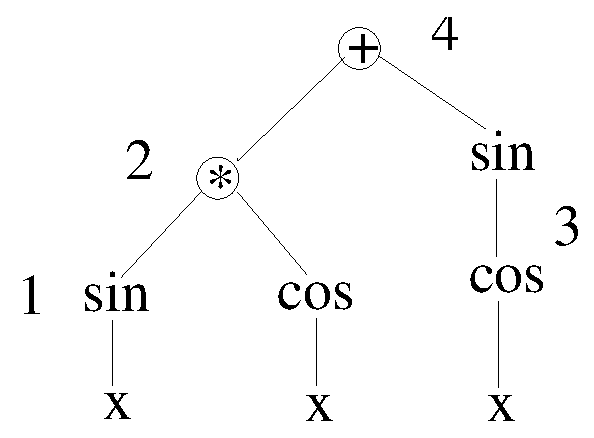
\includegraphics[scale=0.45]{Figs/fig1.ps}
\caption[]{The parsing tree for $f(x)=sin(x)*cos(x) + sin(cos(x))$}
\label{EX1}
\end{center}
\end{figure}


Let $f(x)=sin(x)*cos(x) + sin(cos(x))$ (this includes three
sub-expressions one of which is a functional), represented as a tree
in Fig.~\ref{EX1}.  A value of $1$ is pushed on the \DS\ whenever a
symbol from the symbol-table is pushed on the \VMS.  When branch {\bf
  1} in the above tree is reduced, a call to the built-in function
$sin$ pops a value from the \VMS\ (which is $x$) and a value from the
\DS\ (which is $1$) into two temporary variables, say $t$ and $dt$.
It then pushes the value of $sin(t)$ on the \VMS\ and a value of
$dx*\partial sin / \partial x = dt*cos(t)$ on the \DS.  Similar
operations are done for the branch for evaluating $cos(x)$.  When the
execution reaches node {\bf 2}, the \VMS\ has the values $sin(x)$ and
$cos(x)$ and the \DS\ will have $cos(x)$ and $-sin(x)$.  Since '$*$'
is a binary operator, when node {\bf 2} is reduced, two values, namely
$sin(x)$ and $cos(x)$, from the \VMS\ will be poped.  Two values from
the \DS, namely $cos(x)$ and $-sin(x)$ are also poped.  The
multiplication operator then pushes the result of $sin(x)*cos(x)$ on
the \VMS\ while the result of $cos^2(x)-sin^2(x)$ is pushed on the
\DS\ (note that this uses values from the \DS\ as well as from the
VMS).  Both the stacks now have one value each - \VMS\ the value of
the sub-expression $sin(x)*cos(x)$ and the \DS\ the value of the
derivative of this sub-expression.

Next, branch marked by {\bf 3} will be evaluated.  Again, a value of
$1$ and the value of $x$ is pushed on the \DS\ and the \VMS\ 
respectively.  A call to $cos$ will compute the derivative of $cos(x)$
(namely, $-sin(x)$), multiply the derivative by the top of the \DS\ 
(which is $1$) and push the result on \DS.  A call to $sin$ will do
the same - pop the \DS\ (which has the value $-sin(x)$), multiply by
$\partial sin(cos(x))/\partial (cos(x))$ (namely, $cos(cos(x))$) and
push it on the \DS\ (the value pushed on the \DS\ now is
$-sin(x)*cos(cos(x))$).  This is the equivalent of
Eq.~\ref{DFUNCTIONAL} for branch {\bf 3}.  At this stage, the two
values on the \VMS\ are the values of the two sub-expression and \DS\ 
has the values of the partial derivatives of the two sub-expressions.

Reduction of the node {\bf 4} will then again invoke the rule for the
derivative and the binary operator for addition: pop two values from
the \VMS\ and \DS, push the result of the operator on the \VMS, and
the derivative (addition of the two values from the \DS\ in this case)
on the \DS.  The '{\tt=}' operator would then square the value of the
top of \DS, multiply it by $\delta x^2$, take the square root of the
result and push the result on the \DS\ again (the reason for squaring
and then taking square root will become clear when we discuss the case
of multi-variate expressions).  This leaves the value of $\delta f$
(Eq.~\ref{FERR}) on the \DS.

\section{Error propagation: The general algorithm for multi-variate case}
\label{SEC:MULTI_VAR}

The general algorithm which would work for multi-variate case as well
is similar to the single-variate case described above, but slightly
more complicated.  Multi-variate expressions have the added
complication that the partial derivatives in the summation of
Eq.~\ref{FERR} have to be evaluated separately for {\it each
  independent} variable.  This means that a \DS\ {\it per independent}
variable has to be maintained.  The data structure used for \DS\ is an
array of stacks.  A table of measurement errors ({\tt ME}) associated
with each independent variable is also required.

For the general multi-variate case, symbols (variable or a constant)
in \Fussy\ are tagged with a unique ID and a type.  Symbols
representing normal variables are of type {\tt VAR} and have a single
unique ID, a random error and a partial derivative (of value 1)
associated with them.  Symbols representing sub-expressions are of
type {\tt PARTIAL\_VAR} and have a list of IDs (rather than a single
unique ID) and a corresponding list of random errors and partial
derivatives associated with them.  List of unique IDs and the random
errors of the independent variables in the expression on the
right-hand side (RHS) of the assignment operator constitute the list
of IDs and random errors for the {\tt PARTIAL\_VAR}.  When a symbol
(of either type) is pushed on the \VMS, the entire list of associated
IDs is copied to the ID list of the object on the stack.  The
corresponding random errors and partial derivatives are copied to the
appropriate locations in the {\tt ME} table and pushed on the
appropriate \DS\ respectively.  For example, let the IDs of $x_1$ and
$x_2$ be $1$ and $2$ respectively.  For an expression $x_1 * x_2$, the
result on the top of the \VMS\ will have an ID list of {\tt \{1,2\}}
retaining the information that the result is statistically dependent
on the independent variates $x_1$ and $x_2$.  If this result is
further used as part of another expression, this information will be
used to propagate the chain rule for these variables correctly.

Since any expression is built using basic mathematical operators or
built-in functions, for the purpose of proving that the error
propagation algorithm works for any arbitrary expression, it is
sufficient to prove that the algorithm works for the fundamental
mathematical operators and built-in functions.  Further evaluation of
the partial derivatives using mathematical operators and the final
evaluation of the resulting error is described below as pseudo code
for various mathematical operators (see Appendix~\ref{APPEN:EX} for an
example).  For the description of the algorithm, the following VM
op-codes are used:
\begin{itemize}
\item {\tt push(S)}: instruction to push the symbol or value {\tt S}
containing an intermediate result on the \VMS.
\item {\tt push(S,i)}: instruction to push the symbol or value {\tt S}
on the $i^{th}$ \DS. 
\item {\tt pop()}: instruction to pop a symbol from the \VMS.
\item {\tt pop(DS[i])}: instruction to pop a symbol from the $i^{th}$ \DS.
\end{itemize}
The \DS\ is indexed by the symbol IDs represented by {\tt N} below.
When a symbol from one of the symbol tables is pushed on the \VMS, a
value of 1 is pushed on {\tt DS[N]} and the associated measurement
error is copied into {\tt ME[N]}.  {\tt L} and {\tt R} in the pseudo
code represents the symbols on the left-hand-side (LHS) and right-hand
side (RHS) of the operator respectively.  Two functions $f(x,a)$ and
$g(x,b)$ with one common variable and one non-common variable each are
used as examples in the explanation below.

All the operators described below are binary operators.  They all pop
two values from the top of the \VMS, compute the result by applying
the corresponding operator, store the value in a temporary stack
object, set its ID to the union of the IDs of the operands and push it
on the \VMS.  These operations are shown in the first block of pseudo
code for each operator below.

%\newpage
%
%--------------------------------------------------------------------  
%
\subsection{The multiplication operator}
\begin{verbatim}
   /* Compute the result for the multipication operator */
   R = pop();  
   L = pop();
   S = L*R;
   S.IDList = union(L.IDList, R.IDList);
   push(S);    /* Push the computed value on the VMS.*/
\end{verbatim}
Partial derivatives with respect to all the IDs in the ID lists of the
operands is at the top of the corresponding {\tt DS}.  For all the IDs
common between the two operands, two values are poped from the
corresponding \DS, say {\tt dxR} and {\tt dxL}.  The common IDs
represent the variables which are part of both the operands (here
$x$).  Partial derivatives with respect to these common variables are
then computed as {\tt dxR*L + dxL*R} (equivalent of computing
${f(x,a)} {\partial g(x,b) \over \partial x} + {g(x,b)}{\partial
  f(x,a) \over \partial x}$) and is pushed on the corresponding \DS\ 
(here, {\tt DS[x.ID]}).
\begin{verbatim}
   IDList = intersection(L.IDList, R.IDList);
   for ID in IDList
     {
       dxR = pop(DS[ID]); /* Pop two values from the same DS */  
       dxL = pop(DS[ID]);
       push(dxR*L + dxL*R, DS[ID]);
       L.RemoveID(ID); R.RemoveID(ID);
     }
\end{verbatim}
For the set of non-common IDs, only ${g(x,b)}{\partial f(x,a) \over
\partial a}$ and ${f(x,a)} {\partial g(x,b) \over \partial b}$ needs
to be computed and pushed on the \DS\ corresponding to the unique IDs
(here IDs of $a$ and $b$ respectively).
\begin{verbatim}
   for ID in L.IDList
     {
       dx  = pop(DS[ID]);  /* this is the partial derivative of L */
       push(dx*R,DS[ID]);
     }

   for ID in R.IDList
     {
       dx  = pop(DS[ID]);  /* this is the partial derivative of R */
       push(dx*L,DS[ID]);
     }
\end{verbatim}

%
%-------------------------------------------------------------------------
%
\subsection{The division operator}

As before, the result of the division of the two operands ({\tt L} and
{\tt R}) is pushed on the stack with an ID equal to the union of the
IDs of the two operands.
\begin{verbatim}
   /* Compute the result for the division operator */
   L = pop();  
   R = pop();
   S = L/R;
   S.IDList = union(L.IDList, R.IDList);
   push(S);
\end{verbatim}
As in the case of the multiplication operator, for all IDs common
between {\tt L} and {\tt R}, two values are poped from the
corresponding \DS\ and the partial derivative computed with respect to
the common variable as {\tt (R*dxL - L*dxR)/(R*R)}.  This is
equivalent to computing:
\begin{equation}
{\partial \over {\partial x}}\left[{f(x,a) \over g(x,b)}\right] =
{1 \over g(x,a)^2}\left[{g(x,a) {{\partial f(x,a)} \over  {\partial
x}}} - f(x,a) {{\partial g(x,b)} \over {\partial x}}\right] 
\end{equation}
The computed derivative is pushed on the appropriate \DS\ (here {\tt
DS[x.ID]}).  The common IDs are then removed from the list of the IDs
in {\tt L} and {\tt R} so that they are not considered again in the
differentiation with respect to the other variables.  The pseudo code
for this operation is:
\begin{verbatim}
   IDList = intersection(L.IDList, R.IDList);
   for ID in IDList
    {
      dxR = pop(DS[ID]); 
      dxL = pop(DS[ID]);
      R.RemoveID(ID); L.RemoveID(ID);
      push((R*dxL - L*dxR)/(R*R), DS[ID]);
    }
\end{verbatim}
Next, partial derivatives with respect to each of the non-common
variables are computed (here with respect to $a$ and $b$).  Partial
derivative with respect to $a$ is ${1 \over g(x,b)} {\partial f(x,a)
\over \partial a}$ and with respect to $b$ is $-{f(x,a) \over
{g(x,b)^2}}{\partial g(x,b) \over \partial b}$.  The partial
derivatives of $f$ and $g$ with respect to $a$ and $b$ respectively
are poped from the \DS\ indexed by the the IDs of $a$ and $b$.  The
computed partial derivative is then pushed back on the same \DS.
\begin{verbatim}
   for ID in L.IDList
    {
      dx = pop(DS[ID]); 
      push(dx/R,DS[ID]);
    }

   for ID in R.IDList
    {
      dx = pop(DS[ID]);
      push(-L*dx/(R*R),DS[ID]);
    }
\end{verbatim}

%-------------------------------------------------------------------------
%
\subsection{The addition operator}

The first set of operations is same as that for other operators except
that the value pushed on the \VMS\ is {\tt L+R}.
\begin{verbatim}
   /* Compute the result for the addition operator */
   L = pop();  
   R = pop();
   S = L+R;
   S.IDList = union(L.IDList, R.IDList);
   push(S);
\end{verbatim}
Since the partial derivatives of the expression with respect to the
non-common variables is already on the appropriate \DS, no separate
operation is required for these variables.  The partial derivatives
with respect to the common set of variables is just the sum of the
partial derivatives of the operands (${\partial f(x,a) \over {\partial
x}}$ and ${\partial g(x,b) \over {\partial x}}$ - which are poped from
the \DS\ corresponding to the IDs of the these variables).  The pseudo
code for these operations is:
\begin{verbatim}
   IDList = intersection(L.IDList, R.IDList);
   for ID in IDList /* common IDs in L and R */
     {
       dxL = pop(DS[ID]);
       dxR = pop(DS[ID]);
       push(dxL+dxR, DS[ID]);
       L.RemoveID(ID); R.RemoveID(ID);
     }
\end{verbatim}
%
%-------------------------------------------------------------------------
%
\subsection{The subtraction operator}

The pseudo code for the subtraction operation is functionally same as
that for the addition operator.
\begin{verbatim}
   /* Compute the result for the subtraction operator */
   L = pop();  
   R = pop();
   S = L-R;
   S.IDList = union(L.IDList, R.IDList);
   push(S);

   IDList = intersection(L.IDList, R.IDList);
   for ID in IDList /* common IDs in L and R */
     if (DS[ID].size() > 1)
       {
         dxL = pop(DS[ID]);
         dxR = pop(DS[ID]);
         push(dxL-dxR, DS[ID]);
         L.RemoveID(ID); R.RemoveID(ID);
       }
\end{verbatim}
This is equivalent of computing ${\partial f(x,a) \over {\partial
    x}}-{\partial g(x,b) \over {\partial x}}$.  In addition to the
above operations, the partial derivatives of the RHS operand with
respect to all the non-common variables needs to be negated (here
$\partial g(x,b) / \partial b$).
\begin{verbatim}
   IDList = union(L.IDList, R.IDList);
   for ID in IDList /* unique IDs in L and R */
     if (ID in R.IDList)
       {
         dxR = pop(DS[ID]);
         push(-dxR, DS[ID]);
       }
\end{verbatim}
  
%
%-------------------------------------------------------------------------
%
\subsection{The power operator}

Again, the result of the to-the-power operator ($L^R$), with an ID
equal to the union of {\tt L.ID} and {\tt R.ID} is pushed on the \VMS.
\begin{verbatim}
   /* Compute the result for the power operator */
   L = pop();  
   R = pop();
   S = L^R;
   S.IDList = union(L.IDList, R.IDList);
   push(S);
\end{verbatim}
The partial derivative of the expression with respect to the common
variable (here $x$) is computed using the top two values on the \DS\
and the value of the two operands as:
\begin{equation}
{\partial \over {\partial
x}}\left(f(x,a)^{g(x,b)}\right)=f(x,a)^{g(x,b)} \left[{g(x,b) \over
f(x,a)} {\partial f(x,a)  \over \partial x} + \log(f(x,b)) 
{\partial g(x,b) \over \partial x} \right] 
\end{equation}
The computed derivative is pushed on the appropriate \DS (here {\tt
DS[x.ID]}) and the IDs common to both the operands are then removed
from the list of IDs in both the operators.  The pseudo code for this
operation is:
\begin{verbatim}
   IDList = intersection(L.IDList, R.IDList);
   for ID in IDList
    {
      dxR = pop(DS[ID]); 
      dxL = pop(DS[ID]);
      push((L^R)*((R/L)*dxL + log(L)*dxR),DS[ID]);
      R.RemoveID(ID); L.RemoveID(ID);
    }
\end{verbatim}
The partial derivatives with respect to the non-common set of IDs
correspond to $g(x,b)f(x,a)^{[g(x,b)-1]} {\partial f(x,a) \over
{\partial a}}$ and $f(x,a)^{g(x,b)} \log(f(x,b)) {\partial g(x,b)
\over \partial b}$.  Partial derivatives of $f$ and $g$ with respect
to $a$ and $b$ are poped from the \DS s corresponding to the ID list
of $a$ and $b$ respectively.  The computed partial derivatives are
pushed back on the appropriate \DS.  The pseudo code for this
operation is:
\begin{verbatim}
   for ID in L.IDList
     {
       dxL = pop(DS[ID]); 
       push(R*(L^(R-1))*dxL,DS[ID]);
     }

   for ID in R.IDList
     {
       dxR = pop(DS[ID]); 
       push((L^R)*log(L)*dxR,DS[ID]);
     }
\end{verbatim}
At the terminal operators (e.g. the assignment operator '{\tt =}'), a
single value (the result of the right hand side of the terminal
operator) is poped from the \VMS.  The propagated error is then
computed using the values from the top of all \DS s corresponding
to the IDs in the ID list of the value poped from the \VMS.  The
values from these \DS s are the partial derivatives of the
expression with respect to the various independent variables used in
the expression on the right hand side ($\partial f / \partial x_i$ in
Eq.~\ref{FERR}).  The corresponding measurement errors ($\delta x_i$
in Eq.~\ref{FERR}) are in the appropriated locations in the {\tt ME}
table.  Using these values, Eq.~\ref{FERR} is evaluated.  This is the
final propagated error in the expression.

\section{Examples}
\label{SEC:EXAMPLES}
Following are some examples to demonstrate as well as test the
correctness of the error propagation algorithm of
Section~\ref{SEC:MULTI_VAR}.  In the following examples, various
functions are written in different algebraic forms and the results for
the different forms is shown to be exactly same (e.g. $cos(x)$ vs.
$\sqrt{1-sin^2(x)}$, $tan(x)$ vs. $sin(x)/cos(x)$).  These examples
also verify that the combination of a function and its inverse simply
returns the argument (e.g $asin(sin(x))=x$), as well as functions like
$sinh(x)/((exp(x)-exp(-x))/2)$ (which is really a complicated way of
writing $1$!) returns a value of $1$ with zero error.  However, if the
values of two independent variates $x_1$ and $x_2$ and their
corresponding errors are same, the value of expressions like
$sin^2(x_1) + cos^2(x_2)$ will be $1$ but the error will not be zero.
\begin{verbatim}
   Value of x         =  1.00000 +/- 0.10000
   Value of y         =  2.00000 +/- 0.20000
   Value of x1        =  1.00000 +/- 0.10000
   Value of x2        =  1.00000 +/- 0.10000

   sin(x)             =  0.84147 +/-  0.05403
   sqrt(1-sin(x)^2)   =  0.54030 +/-  0.08415
   cos(x)             =  0.54030 +/-  0.08415

   tan(x)             =  1.55741 +/-  0.34255
   sin(x)/cos(x)      =  1.55741 +/-  0.34255

   asin(sin(x))       =  1.00000 +/-  0.10000
   asinh(sinh(x))     =  1.00000 +/-  0.10000
   atanh(tanh(x))     =  1.00000 +/-  0.10000
   exp(ln(x))         =  1.00000 +/-  0.10000

   sinh(x)            =  1.17520 +/-  0.15431
   (exp(x)-exp(-x))/2 =  1.17520 +/-  0.15431

   sinh(x)/((exp(x)-exp(-x))/2) =  1.00000
   x/exp(ln(x))                 =  1.00000

   sin(x1)*sin(x1)       =  0.70807 +/- 0.09093
   sin(x1)*sin(x2)       =  0.70807 +/- 0.06430
   (sin(x1)^2+cos(x1)^2) =  1.00000 +/- 0.00000
   sin(x1)^2+cos(x2)^2   =  1.00000 +/- 0.12859
\end{verbatim}

\subsection{Recursion}

Following is an example of error propagation in a recursive function.
The factorial of $x$ is written as a recursive function $f(x)$ in
\Fussy.  Its derivative is given by $f(x)\left[\frac{1}{x} +
\frac{1}{x-1} + \frac{1}{x-2} +...+
\frac{1}{2} + 1\right]$.  The second term in this
expression is also written as a recursive function $df(x)$.  It is
shown that the propagated error in $f(x)$ is equal to
$f(x)df(x)\delta x$.
\begin{verbatim}
   >f(x) {if (x==1) return x; else return x*f(--x);}
   >df(x){if (x==1) return x; else return 1/x+df(--x);}
   >x=10pm1
   >f(x)
           3628800.00000 +/- 10628640.00000
   >(f(x)*df(x)*x.rms).val
           10628640.00000
\end{verbatim}

Similarly, the recurrence relations for the Laguerre polynomial of
order $n$ and its derivative evaluated at $x$ are given by
\begin{eqnarray}
&L_n(x)& = \left\{
	\begin{array}{lr}
	1&~~n=0\\
	1-x&~~n=1\\
	\frac{(2n-1-x)L_{n-1}(x)-(n-1)L_{n-2}(x)}{n}&~~n\ge2
	\end{array}
	\right. \\
&L^\prime_n(x)&  = (n/x)\left[L_n(x) - L_{n-1}(x)\right]
\end{eqnarray}
%&L_0(x)&         = 1~~~and~~~L_1(x)=1-x\nonumber \\ 
%&L_{n \ge 2}(x)& = (2n-1-x)L_{n-1}(x)-(n-1)L_{n-2}(x) \\
These are written as recursive functions {\tt l(n,x)} and {\tt
dl(n,x)} and it is shown that the propagated error in $L_n(x)$ is
equal to $L^\prime_n(x)\delta x$.
\begin{verbatim}
   >l(n,x){
      if (n<=0) return 1;
      if (n==1) return 1-x;
      return ((2*n-1-x)*l(n-1,x)-(n-1)*l(n-2,x))/n;
    }
   >dl(n,x){return (n/x)*(l(n,x)-l(n-1,x));}
   >x=3pm1;
   >l(4,x)
               1.37500 +/-    0.50000
   >(dl(4,x)*x.rms).val
           0.50000
\end{verbatim}

\appendix       
\section{Appendix: An example of a multi-variate expression}
\label{APPEN:EX}
Parsing tree for the multi-variate expression $f(x_1,x_2)={x_1\times
x_2+x_1 \over {x_2}}$ is shown in Fig.~\ref{EX2}.  The sequence of
operations at the stages marked by {\bf 1,2} and {\bf 3} are as
follows.  In the following, {\tt <variablename>.rms()} and {\tt
<variablename>.ID} refers to the random error and the ID associated
with the variable respectively.
\begin{figure}[t]
\begin{center}
  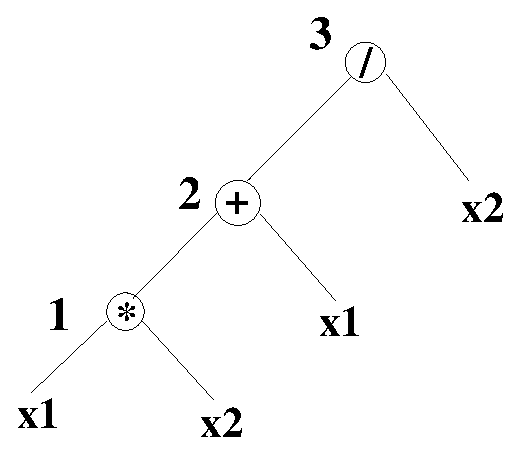
\includegraphics[scale=0.45]{Figs/fig2.ps}
\caption[]{The parsing tree for $f(x_1,x_2)={x_1\times x_2+x_1 \over {x_2}}$}
\label{EX2}
\end{center}
\end{figure}
%\newpage
\begin{enumerate}
\item Stage {\bf 1}:
  
  The IDs of {\tt x$_1$} and {\tt x$_2$} are set to $0$ and $1$
  respectively and they are pushed on the \VMS.  {\tt x$_1$.rms()}
  and {\tt x$_2$.rms()} are copied in {\tt ME[0]} and {\tt ME[1]}
  respectively, while a value of $1$ is pushed on {\tt DS[0]} and {\tt
  DS[1]}.
  

  Operator {\tt '*'} pops two values (say {\tt L} and {\tt R}) from
  the \VMS.  A value {\tt L*R} with an ID equal to {\tt
  L.ID}$~\cup~${\tt R.ID} is pushed on the \VMS\ and a list of common
  IDs is made as {\tt IDList = L.IDList}$~\cap~${\tt R.IDList} (here,
  an empty list).  Next, for all IDs in {\tt L}, a value is poped from
  {\tt DS[L.ID]} (say, {\tt dx}), and {\tt dx*R} is pushed back on
  {\tt DS[L.ID]}.  Similar operation is done for all IDs in {\tt R}.
  
  Top of {\tt DS[0]} and {\tt DS[1]} now has {\tt x$_2$} and {\tt
  x$_1$} respectively, while the top of the \VMS\ has the value
  {\tt x$_1 \times $x$_2$} with an {\tt IDList=\{1,0\}}.

\item Stage {\bf 2}:
  
  {\tt x$_1$} is pushed on the \VMS, its ID is set to zero, {\tt
  x$_1$.rms()} is copied to {\tt ME[0]} (a redundant operation) and a
  value of $1$ is pushed on {\tt DS[0]}.
  
  Operator {\tt '+'} pops two values ({\tt L} and {\tt R}) from the
  \VMS\ (these have values {\tt x$_1\times$x$_2$} and {\tt x$_1$}).
  {\tt L+R} with an {\tt IDList= L.ID}$~\cup~${\tt R.ID} is pushed
  back on the \VMS.  This {\tt IDList} will be {\tt \{0,1\}}.  For IDs
  common between {\tt L} and {\tt R} (here $\{0\}$), two values are
  poped from the \DS, and their addition pushed back on the \DS.  The
  common ID is then removed from the ID list of both operands.  For
  the remaining IDs in {\tt L} ({\tt R} has no IDs left), values are
  poped from the corresponding \DS, added together and pushed
  back on the appropriate \DS.
  
  Hence, at the end of the operator {\tt '+'}, {\tt DS[0]} will have
  {\tt x$_2$+1} and {\tt DS[1]} will have {\tt x$_1$}.  Top of the
  \VMS\ has the value {\tt x$_1 \times$x$_2$+x$_1$}.

\item Stage {\bf 3}:
  
  {\tt x$_2$} is pushed on the \VMS, {\tt x$_2$.rms()} is copied
  in {\tt ME[1]} (another redundant operation) and a value of $1$ is
  pushed on {\tt DS[1]}.
  
  Operator {\tt '/'} pops two values ({\tt L} and {\tt R}) from the
  \VMS.  A value of {\tt L/R} with an {\tt IDList=L.ID}$~\cup~${\tt
  R.ID} ($\{0,1\}\cup\{0\}$) is pushed on the \VMS.  A list of common
  IDs between {\tt L} and {\tt R} is made using {\tt IDList =
  L.IDList}$~\cap~${\tt R.IDList}.  For all IDs in {\tt IDList}, two
  values are poped from the corresponding \DS\ (say, {\tt dxR}
  ({\tt $=$x$_1$}) and {\tt dxL} ($=1$)) and {\tt (R*dxL -
  L*dxR)/(R*R)} pushed back on the same \DS.  The corresponding
  IDs are then removed from {\tt L} and {\tt R}.
  
  Next, for all the remaining IDs in {\tt L}, a value is poped (say
  {\tt dx}) from {\tt DS[L.ID]} and {\tt dx/R} is pushed back on the
  same \DS.  Similarly, for all IDs in {\tt R}, a value from {\tt
  DS[R.ID]} is poped into {\tt dx} and {\tt -L*dx/(R*R)} is pushed
  back on the same \DS.
  
  At the end of this stage, {\tt DS[0]} has the value {\tt 1+1/x$_2$}
  and {\tt DS[1]} has the value {\tt -x$_1$/x$_2^2$}.  \VMS\ now has
  ${{\tt x}_1 \times {\tt x}_2 + {\tt x}_1 \over {\tt x}_2}$.
       
\end{enumerate}

Finally, the values from the top of {\it all} \DS s are multiplied
with corresponding values in {\tt ME} table, squared, added and the
square root of the final result is taken.  That value will be
$\sqrt{\left[\left(1+{1\over {\tt x}_2}\right) \times \delta {\tt
x}_1\right]^2+\left[-{{\tt x}_1 \over {\tt x}_2^2} \times \delta {\tt
x}_2\right]^2}$.  This is the final error propagated through the
expression.

\section{Appendix: Syntax}
\label{APPEN:SYNTAX}

This appendix describes the \Fussy\ syntax.  Statements are
interactively executed as soon as they are completed.  The virtual
code for the sub-programs (function or procedure) is held in the
memory and executed when the sub-programs are called.

\subsection{Numbers}
\label{NUMBERS}
Numbers in \Fussy\ are represented as floating point numbers and can
be specified with or without the decimal point, or in the exponent
format.

Optionally, an error can also be associated with the numbers via the
{\tt pm} directive.  E.g., $75.3\pm 10.1$ can be expressed as {\tt
75.3pm10.1}.  Numbers can also be tagged with units (see
Section~\ref{UNITS}) or a {\tt C}-styled printing format (see
Section~\ref{FORMATTING}).

\subsubsection{Units}
\label{UNITS}
   
Numerical values can be specified along with their units.  As of now,
the only units supported are degree, arcmin, arcsec, hours, minute,
and seconds.  These can be specified by appending {\tt 'd', ''', '"',
'h', 'm', 's'} respectively to the numeric values.  Internally, all
numeric values are always stored in the MKS system of units.  The
default units for a variable used to specify angles or time is
radians.  If the values are specified along with any of the above
mentioned units, the values are still stored internally as radians.
However while printing (see Section~\ref{PRINT}), the values are
formatted automatically and printed with the appropriate units.

\subsection{Operators and built-in functions}

The normal binary operators of type {\tt expr <op> expr} where {\tt
  expr} is any expression/variable/constant and {\tt <op>} is one of
{\tt '$+$', '$-$', '$/$', '$*$', '\^{}'} and {\tt '$**$'} binary
operators perform the usual mathematical operations in addition to
propagating the errors in the result.  The comparison operators {\tt
  '$<$', '$>$', '$=$', '$!=$', '$<=$', '$>=$'} and the logical
operators {\tt '||'} and {\tt '\&\&'} have the usual meaning.  Apart
from the usual operation, the {\tt var=expr} assignment operator also
does the error propagation in the expression on the RHS and assigns it
as the error for the variable on the LHS.  In addition to this, the
assignment operator for partial variables ({\tt pvar:=expr}) is also
defined.  This does not propagate the errors on the RHS but instead
transfers all the required information for error propagation to the
variable on the LHS (see Section~\ref{APPEN:SUBEXPRESSIONS}).  The
result of these assignment operators is the value on the variable on
the LHS.  Hence expressions like {\tt sin(x=0.1pm0.02)} are equivalent
to {\tt 'x=0.1pm0.02;sin(x);'}.  The prefix and postfix operators {\tt
  <op>var} and {\tt var<op>} where {\tt <op>} is either {\tt '$++$'}
or {\tt '$--$'} and {\tt var} is any user defined variable are also
defined.  These increment or decrement the value of the variables by
one.  The prefix operators operate on the variables before while the
postfix operators operate after the variable is further used.

In addition two operators of type {\tt expr.<op>} where {\tt <op>} is
either {\tt val} or {\tt rms} are also defined.  These operators
extract the value and the associated (propagated) error in {\tt expr}
which can be any mathematical expression or a variable.

The following built-in functions are defined: {\tt sin}, {\tt cos},
{\tt tan}, {\tt asin}, {\tt acos}, {\tt atan}, {\tt atan2}, {\tt
sinh}, {\tt cosh}, {\tt tanh}, {\tt asinh}, {\tt acosh}, {\tt atanh},
{\tt exp}, {\tt ln}, {\tt log}, {\tt fabs}, {\tt fmod}, {\tt sqrt}
{\tt int}.

\subsection{Expressions/Statements}
\label{APPEN:SYNTAX_EXPR}

Numbers and variables can be combined with the mathematical operators
and logical operators to form an expression.  Expressions can be used
as arguments to built-in or user defined functions (see
Section~\ref{APPEN:SYNTAX_FUNC}).  An expression followed by a NEWLINE
prints its result on the output stream (see Section~\ref{PRINT}) in
the default format (see Section~\ref{FORMATTING}).

For the purpose of error propagation, the print statement and the
assignment operator (the ``{\tt =}'' operator but not the ``{\tt :=}''
operator; see Section~\ref{APPEN:SUBEXPRESSIONS}) are treated as the
terminal nodes of the parsing tree which invoke the final error
propagation.

Assigning a value to a variable also creates the variable.  The type
of the value assigned to the variable determines its type (and overrides
the value or the type of a previously declared variable).  E.g.
\begin{verbatim}
   >H_0=75pm10
   >H_0
             75.00000 +/-   10.00000
   >H_0="The Hubble's constant\n"
   >H_0
    The Hubble's constant
\end{verbatim}
A semi-colon ({\tt ';'}) is a delimiter to separate multiple
expressions in a single line.  Statements on separate lines need not
be delimited by semi-colons (though it is not an error to do so).
Compound statements are a group of simple statements, grouped using the
curly-brace pair ({\tt '\{'} and {\tt '\}'}) (e.g. {\tt \{a=1.5;
b=2;\}}). As may be obvious, compound statements can also be nested.
The {\tt '/\/*'} and {\tt '*/'} pair can be used as comment
delimiters.  Comment delimiters however cannot be nested. 
%E.g.

\subsection{Sub-expressions}
\label{APPEN:SUBEXPRESSIONS}

A special assignment operator '{\tt :=}' is used to assign
sub-expressions to user defined variables.  Sub-expression variables
are different from normal variables in that their propagated error is
computed on-the-fly when required, i.e.  when they are printed or are
assigned to a normal variable using the '{\tt =}' operator or at an
operator node of a parsing tree when used in another expression.  E.g.
\begin{verbatim}
   >x=1pm0.1
   >s:=sin(x);c:=cos(x);
   >sin(x)/cos(x) /* Compute tan(x) as sin(x)/cos(x) */
       1.55741 +/-    0.34255
   >s/c           /* Compute tan(x) using two PARTIAL_VAR */
       1.55741 +/-    0.34255
   >tan(x)        /* Direct computation of tan(x) */
       1.55741 +/-    0.34255
   >s2=s;
   >s2/c          /* Compute tan(x) with a normal variable
                     and one PARTIAL_VAR.  Error propagates 
                     differently */
       1.55741 +/-    0.26236
\end{verbatim}

\subsection{Variables and function/procedure names}

Variable/function/procedure names can be of any length and must match
the regular expression {\tt [a-zA-Z\_]+[a-zA-Z0-9\_]*}.  That is, the
names must start with an alphabet or {\tt '\_'} and can be followed by
one or more alpha-numeric characters or {\tt '\_'}.

\subsection{Function/procedure}
\label{APPEN:SYNTAX_FUNC}

Sub-programs can be written as functions or procedures.  The only
difference between functions and procedures is that functions {\it
  must} return a value while procedures must {\it not} return a value.
Functions can return values with the {\tt return}~{\tt <expression>}
statement.  If {\tt return} is used within the sub-program body, the
type of the subprogram automatically becomes of the type {\tt func}.
Else the type becomes {\tt proc}.  The type of the sub-program
therefore need not be declared.  It is an error to use a procedure in
an expression or pass a procedure as an argument to another
sub-program where a function should have been passed.

A function or procedure declaration begins with a variable name
followed by an argument list.  The argument list is enclosed by a
round bracket pair ({\tt '('} and {\tt ')'}).  A {\tt '()'} specifies
an empty argument list.  In an interactive session, the parser will
expect the next token to be {\tt '\{'} followed by the sub-program
code followed by the closing {\tt '\}'} bracket.  E.g.
\begin{verbatim}
   >/* An example of a funtion declaration */
   >f()
     {
       return sin(PI/2);
     }
   >/* An example of a procedure declaration */ 
   >p() {print "Value of f() = ",f(),"\n";}
   >f()
              1.00000
   >p() 
   Value of f() =    1.00000
\end{verbatim}
A sub-program can be passed as an argument to another sub-program.  An
argument corresponding to a sub-program can be specified using the
{\tt func} (for a function) or {\tt proc} (for a procedure) directive.
E.g.
\begin{verbatim}
   >f(x) { return sin(x); }
   >p(func fa,x) {print "The value of f(",x%5.2f,") =",fa(x),"\n";}
   >p(f,10)
   The value of f(10.00) =  -0.54402
\end{verbatim}
All symbols (variables, functions, procedures) used in the sub-program
code must be either global variables declared {\it before} the
sub-program declaration begins or must be one of the argument list.
Temporary variables, the scope of which is within the sub-program
only, can be declared using the {\tt auto} directive.  E.g.
\begin{verbatim}
   >f(x) { return sin(x); }
   >p(func fa,x)
     {
       auto t;
       t=fa(x);
       print "The value of f(",x%5.2f,") =",t,"\n";
     }
   >p(f,10)
   The value of f(10.00) =  -0.54402
\end{verbatim}


\subsection{Control statements}

The {\tt if-else}, {\tt while-} and {\tt for-}loops constitute the
program control statements.  These loops can be broken at any stage
with the use of the {\tt break} statement.  As of now, the conditions
which control the logic is evaluated ignoring the error with the
control variables.  Ultimately the goal is to provide a language
feature to specify a significance level and the conditional statements
return true if the error on the evaluated value is within the
significance level, else return false.

\subsubsection{{\tt if-else}}

The syntax for the {\tt if-else} statement is:
\begin{verbatim}
    if (condition)
       if-body-statment
    
         or

    if (condition)
       if-body-statment else
       else-body-statment
\end{verbatim}
The {\tt if-body-statement} and the {\tt else-body-statement} can be
any valid compound or simple statement.  In case of a simple
statement, the terminating semi-colon is necessary.

\subsubsection{{\tt while-loop}}

The syntax for the {\tt while-loop} is:
\begin{verbatim}
    while (condition)
       body-statment
\end{verbatim}
The {\tt body-statement} can be either a simple or a compound
statement and in case it is a simple statement, the terminating
semi-colon defines the end of the loop.

\subsubsection{{\tt for-loop}}

The syntax for the {\tt for-loop} is:
\begin{verbatim}
    for (init;condition;incr)
      body-statment
\end{verbatim}
where {\tt init} is a comma ({\tt ','}) separate list of simple
statements for initializing the loop variables.  E.g. {\tt init} can
be {\tt i=0,j=0,k=0}. {\tt condition} is a simple, single conditional
statement while {\tt incr} is a list of comma separated
statement(s). The {\tt body-statement} can be any valid simple or
compound statement.  {\tt init} statements are executed first followed
by the {\tt condition} statement.  If the result of the {\tt
condition} statement is non-zero (logical true), the {\tt
body-statements}, the {\tt incr} statement(s) and {\tt condition}
statement are executed in a sequence till the result of the {\tt
condition} statement is zero (logical false).  E.g. following is a
valid {\tt for-loop} with 3 loop-variables, only one of which is
checked in the condition:
\begin{verbatim}
    for (i=0,j=0,k=0;i<10;i=i+1,j=j+1;k=k+1) 
       print "i= ",i," j= ",j," k= ",k,"\n";
\end{verbatim}

\subsection{Print statement}
\label{PRINT}

The {\tt print} statement takes a comma separated list of objects to
be printed.  These objects can be quoted-strings, variables,
constants, condition statements or user defined function names.  The
list can consist of any number of objects and is terminated by a
semi-colon.  The format in which the numeric values are printed is
defined by the format modifier associated with the values (see
Section~\ref{FORMATTING}).  All escaped-characters used in C-styled
printing have the same effect as in the output of the C-styled {\tt
printf} statement.

\subsection{Formatting}
\label{FORMATTING}

Values can be formatted for printing in a variety of ways.  The format
in which a variable is printed is associated with the variable and
consists of a {\tt printf} styled formatting string (with extensions
for specifying the units of the numerical values as well).  E.g., if
{\tt x=75pm10}, by default it will be printed using the {\tt
'\%10.5f'} format.  The default print format can be modified using the
{\tt '.'} operator on a variable.  E.g., one can fix the default print
format of {\tt x} to {\tt '\%5.2f'} by {\tt x.=\%5.2f}.

The print format of a value can also be temporarily modified by
specifying the format along with the variable/value.  E.g. the value
of {\tt x} can be printed in the exponent format as {\tt print x\%E}
or in the in hexadecimal format as {\tt print x\%x}.

An extra formatting, not available in {\tt printf} formatting, is that
of printing the individual bit values using the {\tt \%b} format.
With this, the value is printed in binary (1 or 0) format.  {\tt
\%B} does the same thing except that it prints a space after every 8 bits.
Before printing, the value is casted into a {\tt unsigned long}
integer.
\begin{verbatim}
   >x=10;x%B
        00000000 00000000 00000000 00001010
\end{verbatim}
If the units of a value are specified, the print format is also
appropriately modified.  The only physical units currently supported
are that for time and angles.  Their print format is automatically set
to {\tt \%hms} or {\tt \%dms} respectively.


\begin{acks}
I thank Divya~Oberoi, Rajiv~K.~Singh and R.V.~Urvashi for many useful
discussion I had with them for this work.  This work was started and
largely done while I was working at the National Center for Radio
Astrophysics (NCRA) of the Tata Institute of Fundamental Research
(TIFR), Pune, India and continued at my current position at the
National Radio Astronomy Observatory (NRAO), Socorro, USA.  Support
from NCRA and NRAO is gratefully acknowledged.  All of this work was
done on computers running the GNU/Linux operating system and I wish to
thank the numerous contributors to this software.
\end{acks}

%\begin{thebibliography}{acmtrans}
\bibliographystyle{acmtrans}
\bibliography{fussy}
%\end{thebibliography}

\begin{received}
Nov. 2003
\end{received}
\end{document}


You may wish to know that EDA is a commercial application, marketed by
Wolfram Research Inc., the inventor and vendor of Mathematica. It was
written by David Harrison, Department of Physics, University of
Toronto, in 1995-1996. This brief introduction to using EDA for
propagation of errors was written by David Harrison, September 1998.

%\subsection{Built-in functions and constants}

%Apart from the mathematical functions (mostly defined in {\tt math.h}
%but not all implemented), there are a few more built-in functions and
%constants defined which are of use for astronomical calculations.

%\subsubsection{Functions}
%\begin{enumerate}
%\item {\tt time()}: This returns the current time (the value of the
%      computer's Real Time Clock (RTC)).  The value is return in units of
%      radians (so can be directly used in trigonometric functions),
%      and the format string is set to ``{\tt \%hms}'' (so that it is
%      display in human readable units).
      
%\item {\tt lst()}: This returns the current Local Sidereal Time at the
%      Longitude value in the internal variable named ``{\tt
%      LONGITUDE}''.  This is by default set to {\tt $74^\circ 03^\prime
%3.6^{\prime\prime}$}
%      (the longitude of Pune, India).  This value can be changed using
%      the function {\tt setlong} (see below).

%\item {\tt setlong(Long)}:  This sets the value of the interval
%      variable {\tt LONGITUDE}.  This variable is normally read-only
%      (i.e., can be read and used in expression like any other
%      variable, but its value can not be set).

%      The argument {\tt Long} is the new value supplied by the user in
%      radians (e.g.  {\tt setlong(54d)} will set the value of {\tt
%      LONGITUDE} to $54^\circ$).

%\item {\tt mjd()}:  This returns the value of Modified Julian Day (MJD).

%\item {\tt fmjd()}: This returns the value of the fractional MJD.
      
%\item {\tt day()}: This returns the day of the month as known to the
%      computer RTC.

%\item {\tt month()}: This returns the current month of the year as
%      known to the computer RTC.

%\item {\tt year()}: This returns the current year as known to the
%      computer RTC.
%\end{enumerate}

%\subsubsection{Constants}
%Following constants are also defined.  The can are read-only objects
%which can be used in expression like normal variables but who's values
%cannot be altered by the user (unless there is a built-in function
%supplied to allow the users to alter its value).

%\begin{enumerate}
%\item {\tt PI}:  The value of $\pi$ ($3.141592653589793116$).
%\item {\tt C}:   The value of speed of light ($299792458.0$m/s).
%\item {\tt R2D}: The multiplicative value to convert radians to degree
%($57.295779513082322864$).
%\item {\tt D2R}: The multiplicative value to convert degree to radians.
%\item {\tt A2R}  The multiplicative value to convert from arc second
%to radians.
%\item {\tt H2R}: The multiplicative value to convert from hours of
%time to radian.
%\item {\tt R2H}: The multiplicative value to convert from radians to
%hours of time.
%\item {\tt kb}:  The Boltzmann constant ($1.380470\times10^{-23}$).
%\item {\tt PC2M}: The multiplicative value to convert from parsec to
%meters ($3.085678\times 10^{16}$).
%\item {\tt PC2LY}: The multiplicative value to convert from parsec to
%Lightyear ($3.261633$).
%\item {\tt AU2M}: The multiplicative value to convert from
%Astronomical Units (AU) to meters ($1.495979\times 10^{11}$).
%\item {\tt LONGITUDE}: The value of longitude used in astronomical
%computations (default: $74^\circ03^\prime3.6^{\prime\prime}$).
%\item {\tt LATITUDE}: The value of latitude used in astronomical
%computations (default: $19^\circ04^\prime48^{\prime\prime}$).
%\item {\tt sigma}: The level of statistical significance for fuzzy
%computations (this is not yet used internally).
%\end{enumerate}


http://www.cdrnet.net/projects/nmath/: Math.NET for symbolic
mathematical operations.

http://www.xemacs.org/Documentation/packages/html/calc.html
